\documentclass[conference]{IEEEtran}
\IEEEoverridecommandlockouts
% The preceding line is only needed to identify funding in the first footnote. If that is unneeded, please comment it out.
\usepackage{cite}
\usepackage{amsmath,amssymb,amsfonts}
\usepackage{algorithmic}
\usepackage{graphicx}
\usepackage{textcomp}
\usepackage{xcolor}
\usepackage{hyperref}
\usepackage{listings}
\usepackage{float}
\usepackage{todonotes}

\def\BibTeX{{\rm B\kern-.05em{\sc i\kern-.025em b}\kern-.08em
    T\kern-.1667em\lower.7ex\hbox{E}\kern-.125emX}}

\newcommand{\arrowright}{$\,\to\,$}
    
\begin{document}

\title{App-controlled LEGO robotic arm\\
{\footnotesize Project of lecture ''Mobile Computing'' (winter term 2018/2019)}
}

\author{
\IEEEauthorblockN{Christoph Ulrich}
\IEEEauthorblockA{%\textit{dept. name of organization (of Aff.)} \\
\textit{HTWG Konstanz}\\
Constance, Germany\\
christoph.ulrich@htwg-konstanz.de}
\and
\IEEEauthorblockN{Benjamin Schaefer}
\IEEEauthorblockA{%\textit{dept. name of organization (of Aff.)} \\
\textit{HTWG Konstanz}\\
Constance, Germany\\
benjamin.schaefer@htwg-konstanz.de}
}

\maketitle

\begin{abstract}
it's reasonable to write this after all other sections of this paper have been completed
\end{abstract}

%\begin{IEEEkeywords}
%component, formatting, style, styling, insert
%\end{IEEEkeywords}\

\section{Introduction / Motivation}
\begin{itemize}
	\item control of a robotic arm is a fundamental task in robotics - easy hands-on experience for everybody to this fundamental robotic application with this paper and the created low cost LEGO 3-DoF (\textit{Degrees of Freedom}) robot arm  (incl. instructions)
	\item application and hardware could be used in basic lecture "Grundlagen der mobilen Robotik" to better understand robot kinematics, ROS and a bit of perception
	\item recycling of old and unused hardware of the robotics lab at the HTWG Konstanz
	\item typical industrial applications to control a robotic arm run on more powerful hardware and often offer a complicated and - for beginners - confusing GUI, \todo[author=Christoph, inline]{insert example(s)} so we developed an easy to use mobile application for Android platforms
	\item ROS because widely used, very modular/extensible and basic framework which almost every student starting with robotics has to get in touch with
\end{itemize}
\par

\todo[author=Christoph, inline]{new paragraph - description of background and main ''problem''}
\begin{itemize}
	\item which platform to choose for controlling the  arm and driving the motors (Arduino, Raspberry, etc.) - should consume as little energy as possible,  should be flexible and portable
	\todo[author=Christoph, inline]{note that in \ref{sec:platform}}
	\item another aspect \arrowright how should the application on the mobile device communication with the controlling device \arrowright BT, WiFi, (lost of steering commands due to radio lacks etc.)
	\item arm construction \arrowright not too many components, not too heavy so that the motors are able to drive the arm even with more than one joint and with gripper load (to demonstrate gripping)
	\item app \arrowright 
\end{itemize}
Constructing a robot arm generally leads to some difficulties.

\section{State of the Art}

\todo[author=Beide, inline]{find two or three example applications/hardware compontents, analyze and compare them, also look at mobile application programming techniques used in these works}
\begin{itemize}
	\item https://ieeexplore.ieee.org/abstract/document/7192973
	\item https://www.hackster.io/slantconcepts/control-arduino-robot-arm-with-android-app-1c0d96
	\item https://www.instructables.com/id/Robot-Arm-Arduino-App/
	\item https://www.kuka.com/en-us/products/robotics-systems/software/application-software/kuka-hrc-guide-app
\end{itemize}

\section{Proposed Approach}\label{sec:approach}

\subsection{Requirements Engineering}\label{sec:requirements}
\todo[author=Beide, inline]{what should the arm be able to achieve in the end? How should the app look like and which functions does it have to provide?}
The app should have the ability to control the arm via a graphical interface. To control the joints individually, there should also be a possibility to adjust the individual joints via buttons or sliders. Since the servomotors are likely to drift there should be a way to recalibrate the arm at any time.
\\\\
The arm should be able to lift smaller 3D printed objects.

\subsection{Platform Decision}\label{sec:platform}
Since the arm and the app should be used for teaching, there was a variety of hardware to choose from. In addition, one goal was to use existing and disused hardware. Thus, the decision quickly on the NXT bricks of Lego Mindstorm [1]. There are enough bricks as well as sensors and motors in the lab. In addition, from the existing Lego technology also the arm can be constructed. Since Lego Technic is made of lightweight plastic, the finished arm can also be taken to a lecture and presented.\\
There was also a choice of Raspberry Pi's or Arduinos, but here it would have been necessary to order hardware such as motors or parts for the arm.\\
Thus, it offered to use the Lego NXT's, since no hardware needs to be ordered here and disused hardware is used again.

\subsection{Arm Construction}\label{sec:construction}
\begin{figure}[bt] 
	\centering
	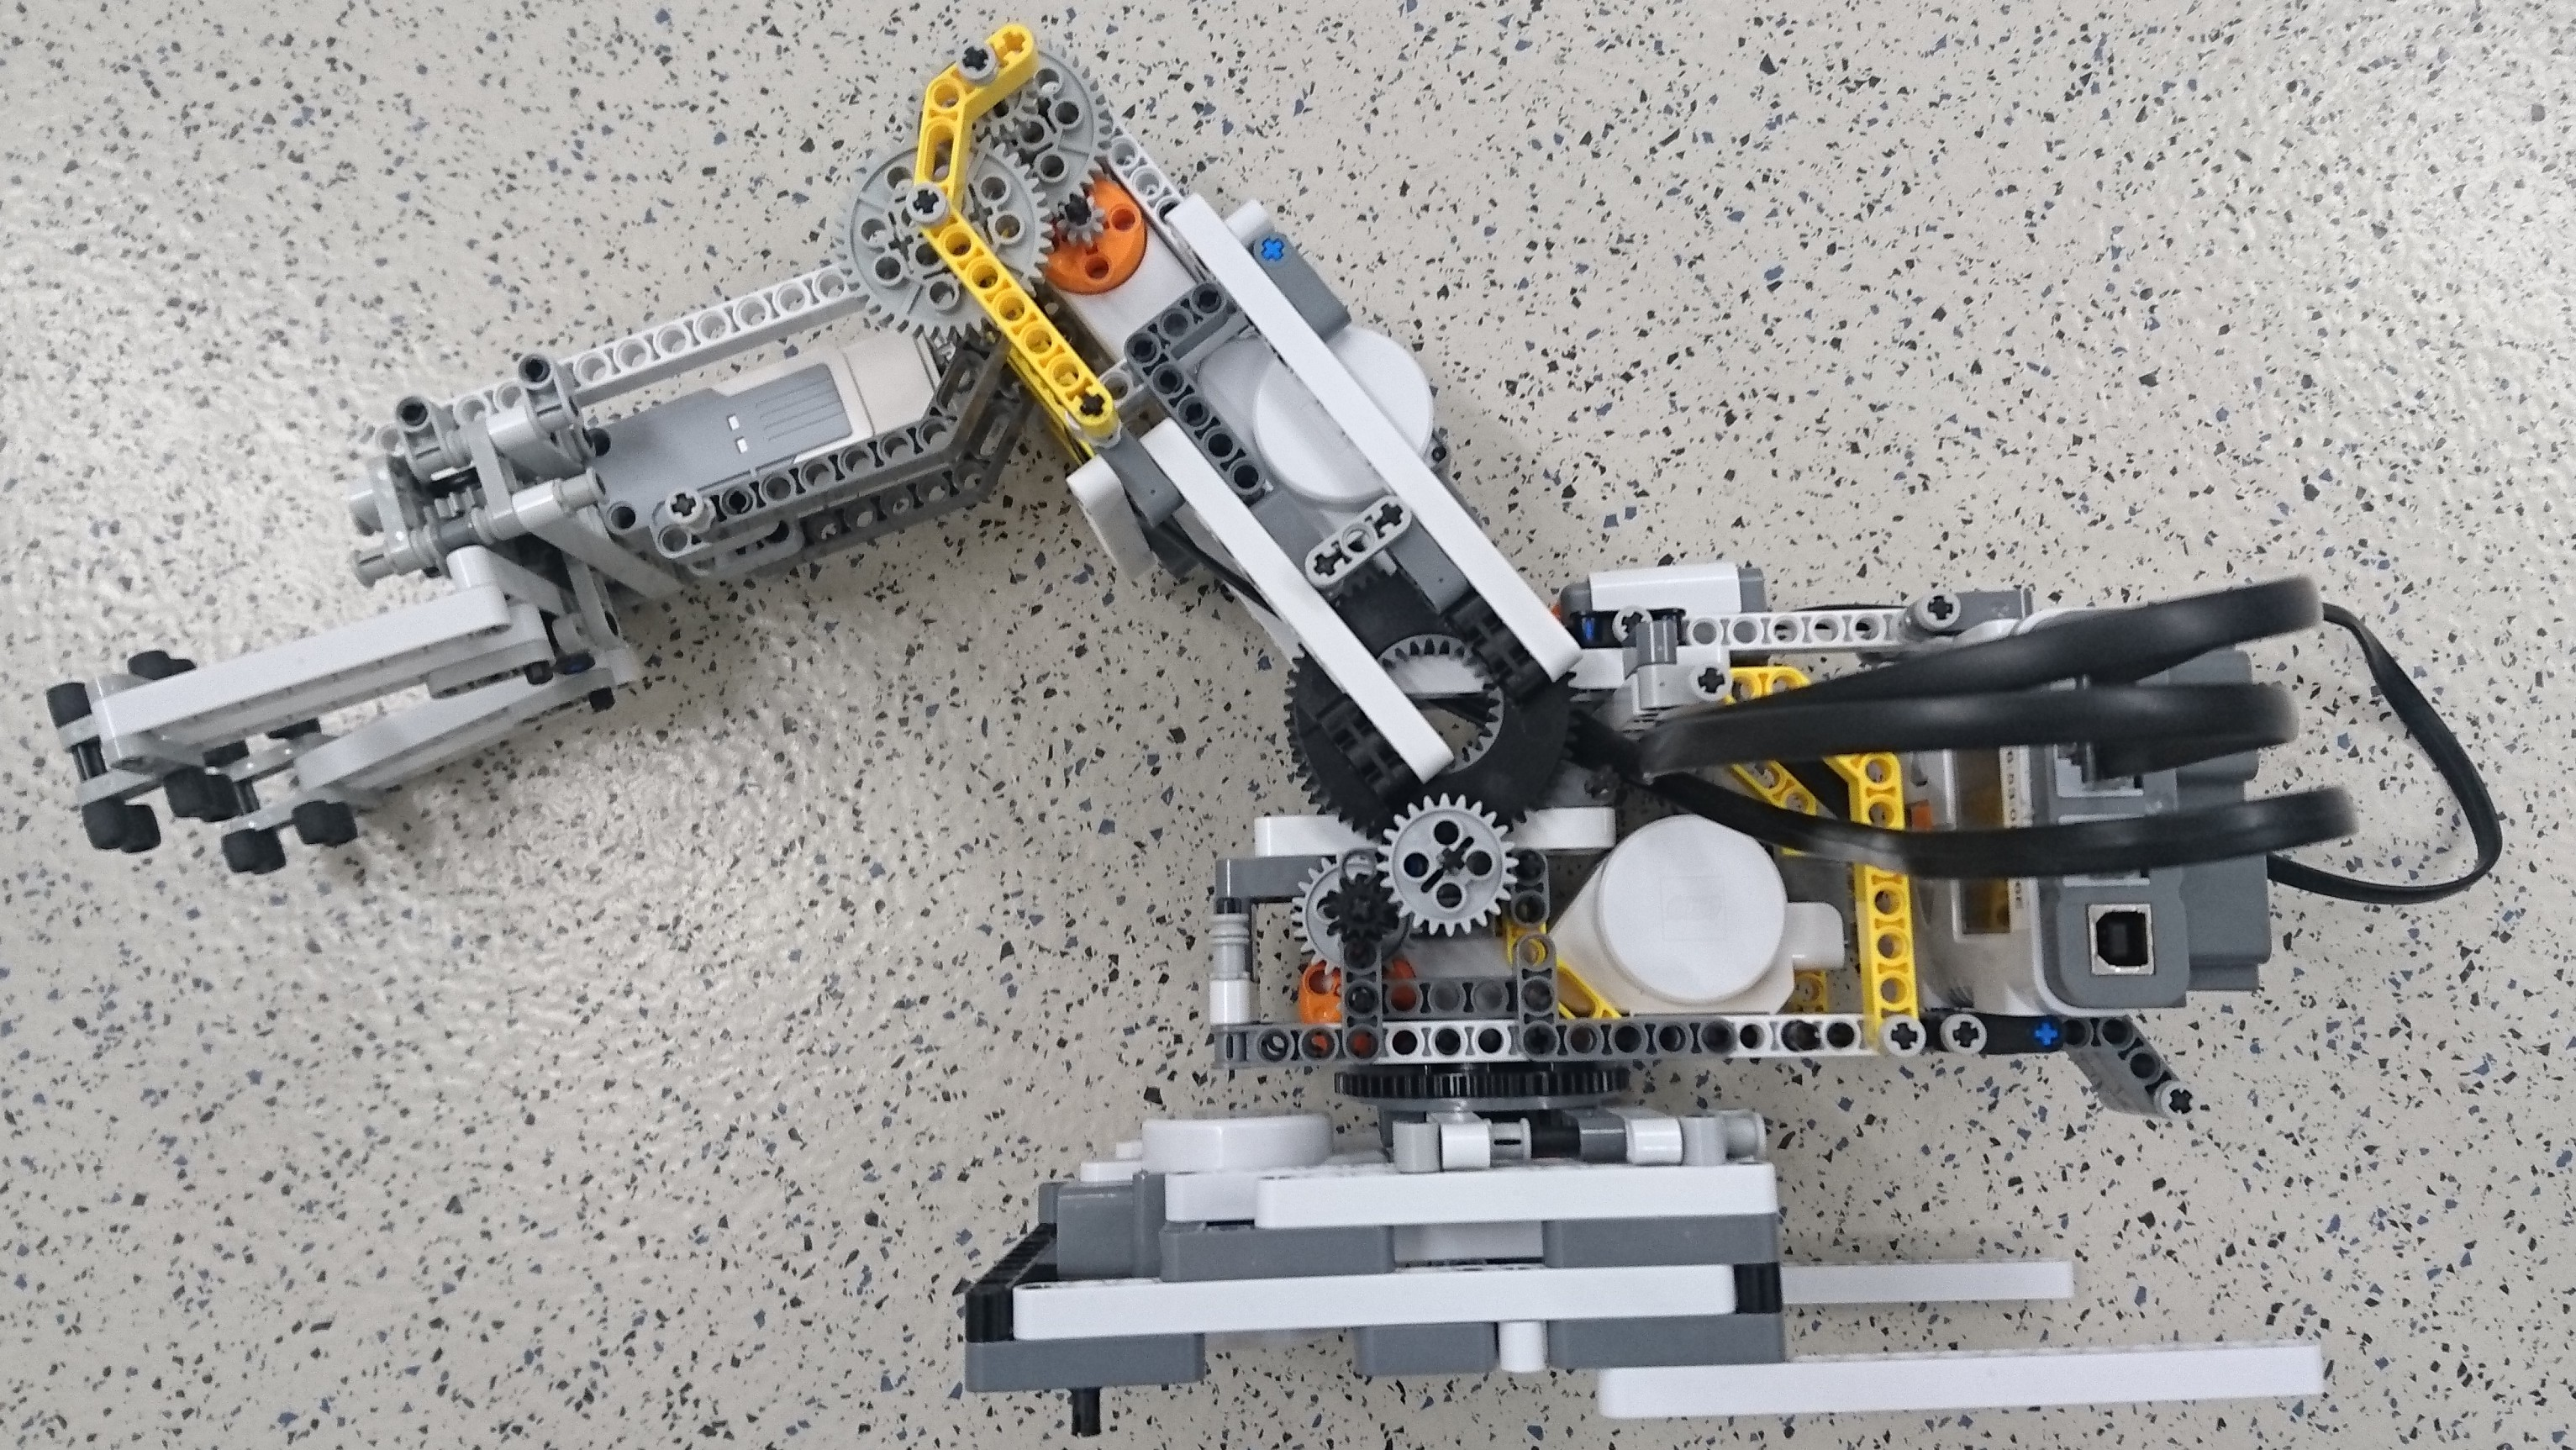
\includegraphics[width=\textwidth/2]{img/arm_full}
	\caption[caption]{Figure of the Lego Technic arm. The lower joint is marked in red and the upper joint in blue}
	\label{fig:arm_full}
\end{figure}
\begin{figure}[bt] 
	\centering
	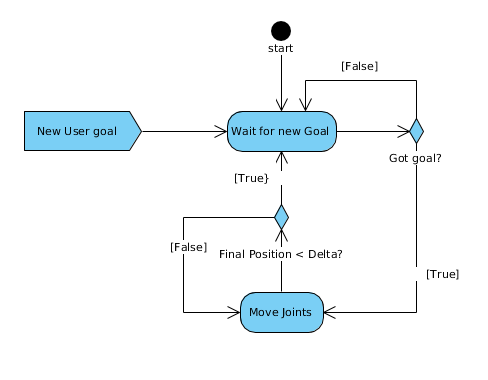
\includegraphics[width=\textwidth/2]{img/control_arm.png}
	\caption[caption]{Activity diagram of the Arm}
\label{fig:activitiy_arm}
\end{figure}

The arm, which can be seen in Figure 1, was designed entirely from Lego Technic. For this purpose, 2 NXT bricks were used. In addition, 4 motors and a touch sensor were used. An NXT was used to control the two arm joints, as well as the gripper. Since the NXTs only have three ports for motors, a second NXT was needed to rotate the base.\\
The servomotors have a built-in rotation sensor with an accuracy of 1 degree. Since these servomotors only have a torque of about 12 N.cm, a translation has been built into the wrist joint so that the motors can move the arm. For this purpose, a translation of 1/42 was used at the lower joint (red circle). The engine's ratio at the upper joint (blue circle) was 2/25.\\
In order to keep the arm as light as possible and to relieve the engines, sensors on the arm itself were completely dispensed with. However, since the engines have to be initialized, a touch sensor has been installed on the base to initialize the first arm articulated. The initialization of the second joint was solved by the torque of the motors, as there is less weight of the arm.

\subsection{Algorithms}\label{sec:algorithms}
\begin{figure}[bt] 
	\centering
	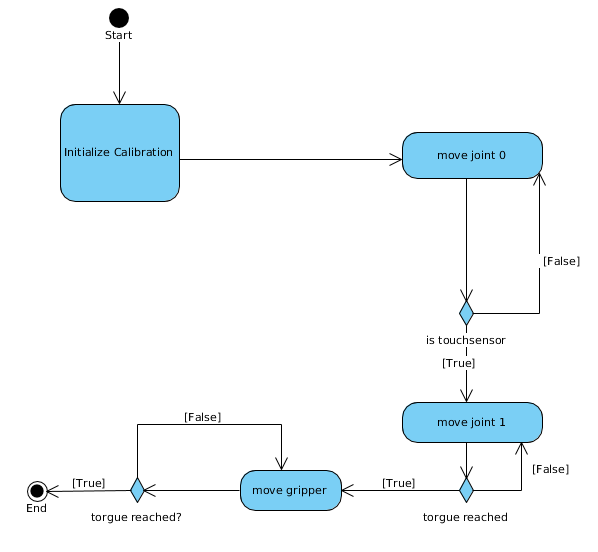
\includegraphics[width=\textwidth/2]{img/calibration.png}
	\caption[caption]{Activity diagram of the calibration process}
\label{fig:calibration}
\end{figure}
The following describes the calibration procedure, which is shown in Figure 2. Since the servomotors can only be controlled by the effort and have no encoder, the starting position of the motors is unknown. Therefore, these must be calibrated. A touch sensor is used for the lower joint. The lower motor rotates until the touch sensor responds to a touch. Then the upper arm is calibrated. Here, the engines rotate with the least force so long, with which the motors can just turn until the joint is in the final position and the engines can not turn, because the effort is too great. In order not to burden the motors unnecessarily, the calibration process is terminated as soon as a certain delta has been exceeded. Finally, the same procedure is repeated for the gripper.
\todo[author=Christoph, inline]{implementation of forward and backward kinematics }
\subsubsection{Kinematics}\label{sec:kinematics}
In order to control the arm it is essential to solve either it's forward or backward kinematics. For our application, we need both problems to be solved. Users of the application should be able to directly control each joint individually (forward kinematics) as well as to move the TCP into a desired position (backward kinematics). We will first take a look at the calculation of the forward kinematics and then introduce a short geometric solution of the backward kinematics for our 3-DoF arm.
\todo[author=Christoph, inline]{TCP - list of abbreviations may be necessary}
\todo[author=Beide, inline]{measurement of arm dimensions}
\par
The goal of forward kinematics is to determine the pose (position and orientation) of the TCP for a given set of joint angles. The pose of the TCP regarding the origin of the robot arm can be described as a concatenation of $n$ transformations, where $n$ is the number of joints, of which every one has its own coordinate system. For our case $n$ is 3:
\begin{equation}\label{eq:trans_matrix}
T_0^3 = T_0^1 * T_1^2 * T_2^3
\end{equation}
where $T_i^{i-1}$ is a transformation matrix according to the \textit{Denavit-Hartenberg} convention:
\begin{equation}\label{eq:dh-convention}
T_i^{i-1} = Tl(0,0,d_i) * R(z, \theta_i) * Tl(a_i,0,0) * R(x, \alpha_i)
\end{equation}
with $Tl$ being a translation matrix, $R$ a rotation matrix, $d_i$ a translation in z, $a_i$ a translation (for prismatic joints) in x, $\theta_i$ a rotation around z and $\alpha_i$ a constant tilt angle between both joints. In our case we don't use prismatic joints and there are no constant tilt angles between the joints (they are all variable). So equation \ref{eq:dh-convention} simplifies to 
\begin{equation}\label{eq:dh-convention-short}
T_i^{i-1} = Tl(0,0,d_i) * R(z, \theta_i)
\end{equation}
By solving equation \ref{eq:dh-convention-short} we get the following transformation matrix $T_i^{i-1}$ for the forward kinematics:
\[
\begin{matrix}
\cos(\theta_i) & -\sin(\theta_i) & 0 & l_i \cdot \cos(\theta_i)  \\
\sin(\theta_i) & \cos(\theta_i) & 0 & l_i \cdot \sin(\theta_i) \\
0 & 0 & 1 & 0 \\
0 & 0 & 0 & 1
\end{matrix}
\]
Finally, one generally can get the pose of the TCP in the world coordinate system (usually that means with reference to the coordinate system of the robot's base) by multiplying the concatenated transformation matrix \ref{eq:trans_matrix} built from the set of given joint angles $\theta_i$ and the known lengths of the arm parts $l_i$ with the origin of the base:
\begin{equation}\label{eq:tcp_goal}
p_{tcp} = T_0^3 * \begin{pmatrix}0\\0\\0\\1\end{pmatrix}
\end{equation}
Note that one have to use homogeneous coordinates here. Also one should remember that $p_{tcp}$ is the pose of the TCP-origin. Usually users want to get the gripping point of their tool - in this case just add the half of the gripper length to the x-direction to the vector in equation \ref{eq:tcp_goal}.
\\
\par

Vice versa, the goal of backward kinematics is to calculate a set of joint angles from a desired TCP-pose. $\chi$

\begin{itemize}
	\item generally for actual 3 dof
	\item visualization and control over 2 dof, separate control of base and gripper
\end{itemize}

\begin{figure}[htbp]
	\centerline{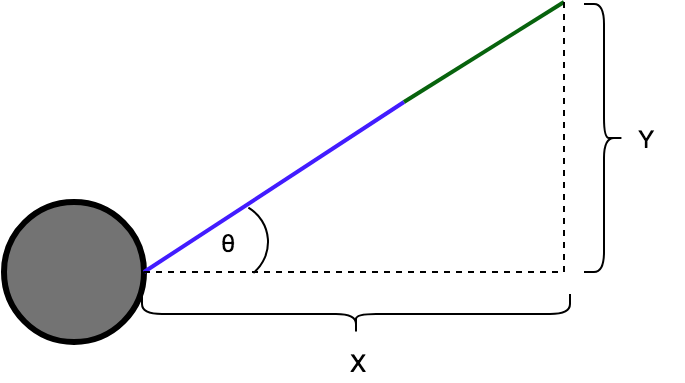
\includegraphics[scale=0.3]{img/kin_yaw_top_view.png}}
	\caption{Top view of the robot. Rotation angle of base joint can be easily calculated with the arctan.}
	\label{fig:yaw_calc}
\end{figure}

\begin{figure}[htbp]
	\centerline{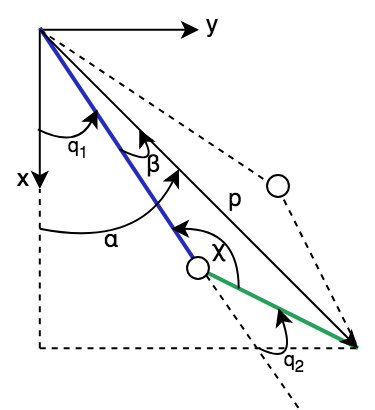
\includegraphics[scale=0.3]{img/kin_q1_q2.png}}
	\caption{Top view of the robot. Rotation angle of base joint can be easily calculated with the arctan.}
	\label{fig:q1_q2_calc}
\end{figure}

\subsection{App Development}\label{sec:development}
\todo[author=Christoph, inline]{communication/process description, ROS, navigation strategy, ... }

\subsection{Expected Results}\label{sec:expectedresults}
\todo[author=Christoph, inline]{speed, accuracy, ...}

\section{Results}

\section{Conclusion}
The NXT can be used to control a robot arm with a smartphone from a remote location. The present scenario has several disadvantages, e.g. Restrictions for cables and the additional computer.
By using ROS this scenario can be extended quickly, eg. by multiple users or a second arm. Despite the rather coarse Lego Technic parts, the arm has a relatively high accuracy and is ideal for demonstrations or teaching.

\section{Further Work}
\begin{itemize}
	\item 3D graphics in App
	\item EV3
	\item algorithms
	\item external better sensors to optimize
\end{itemize}
In further work, the NXT could be exchanged for an EV3. On the one hand, this one more port, which can be 1 NXT saved. On the other hand, the EV3 offers a WiFi interface, which eliminates the need for a laptop for the connection between smartphone and arm.
Currently the app offers only a 2D view of the arm. For a better operation a 3D view could be developed.
Another important point would be to install more and better external sensors to achieve a higher positional accuracy of the arm.

\begin{thebibliography}{00}
\bibitem{onlLegoMindstorm} 
Lego Mindstorm - NXT,
\\\texttt{https://www.lego.com/de-de/mindstorms/downloads/nxt-software-download}
\bibitem{onlROS} 
ROS - Kinetic,
\\\texttt{http://wiki.ros.org/kinetic/Installation}
\bibitem{onlHackster} 
Arduino-Arm with android-app,
\\\texttt{https://www.hackster.io/slantconcepts/control-arduino-
	robot-arm-with-android-app-1c0d96}
\bibitem{onlArduinoArm} 
Robot-Arm-Arduino,
\\\texttt{https://www.instructables.com/id/Robot-Arm-Arduino-
	App/}
\bibitem{onlKuka}
Kuka-hrc-guide,
\\\texttt{https://www.kuka.com/en-us/products/robotics-
	systems/software/application-software/kuka-hrc-guide-
	app}
\end{thebibliography}

\listoftodos

\end{document}